\chapter{Simulation Development}

This chapter describes a software package, \textit{oprc\_env,} that simulates the coverage scenario described in the introduction. This software exposes a standard interface, the \textit{Policy} typeclass, that allows for interaction between the simulation and a wide variety of control algorithms. The package also includes functionality to generate large environment datasets based on custom mixture distributions of environment generation algorithms. oprc\_env also includes functionality to run large batches of simulations with policies that are capable of modifying themselves between scenarios, thereby enabling the development and testing of online machine learning approaches to this problem. Finally, the package features a replay animation utility to aid in communicating results visually. In addition to describing these utilities, this chapter will specify many of the implementation details required to fully understand the coverage scenario and problem statement used in this research.

Note: names of datatypes, type constructors, and type constants in oprc\_env start with capital letters, e.g. Position. For brevity, the names of these datatypes may be used throughout this chapter and the next in reference to both the computational abstractions and the concepts they model.

%get rid of the online machine learning thing if I don't end up doing any of that

\begin{figure}[H]
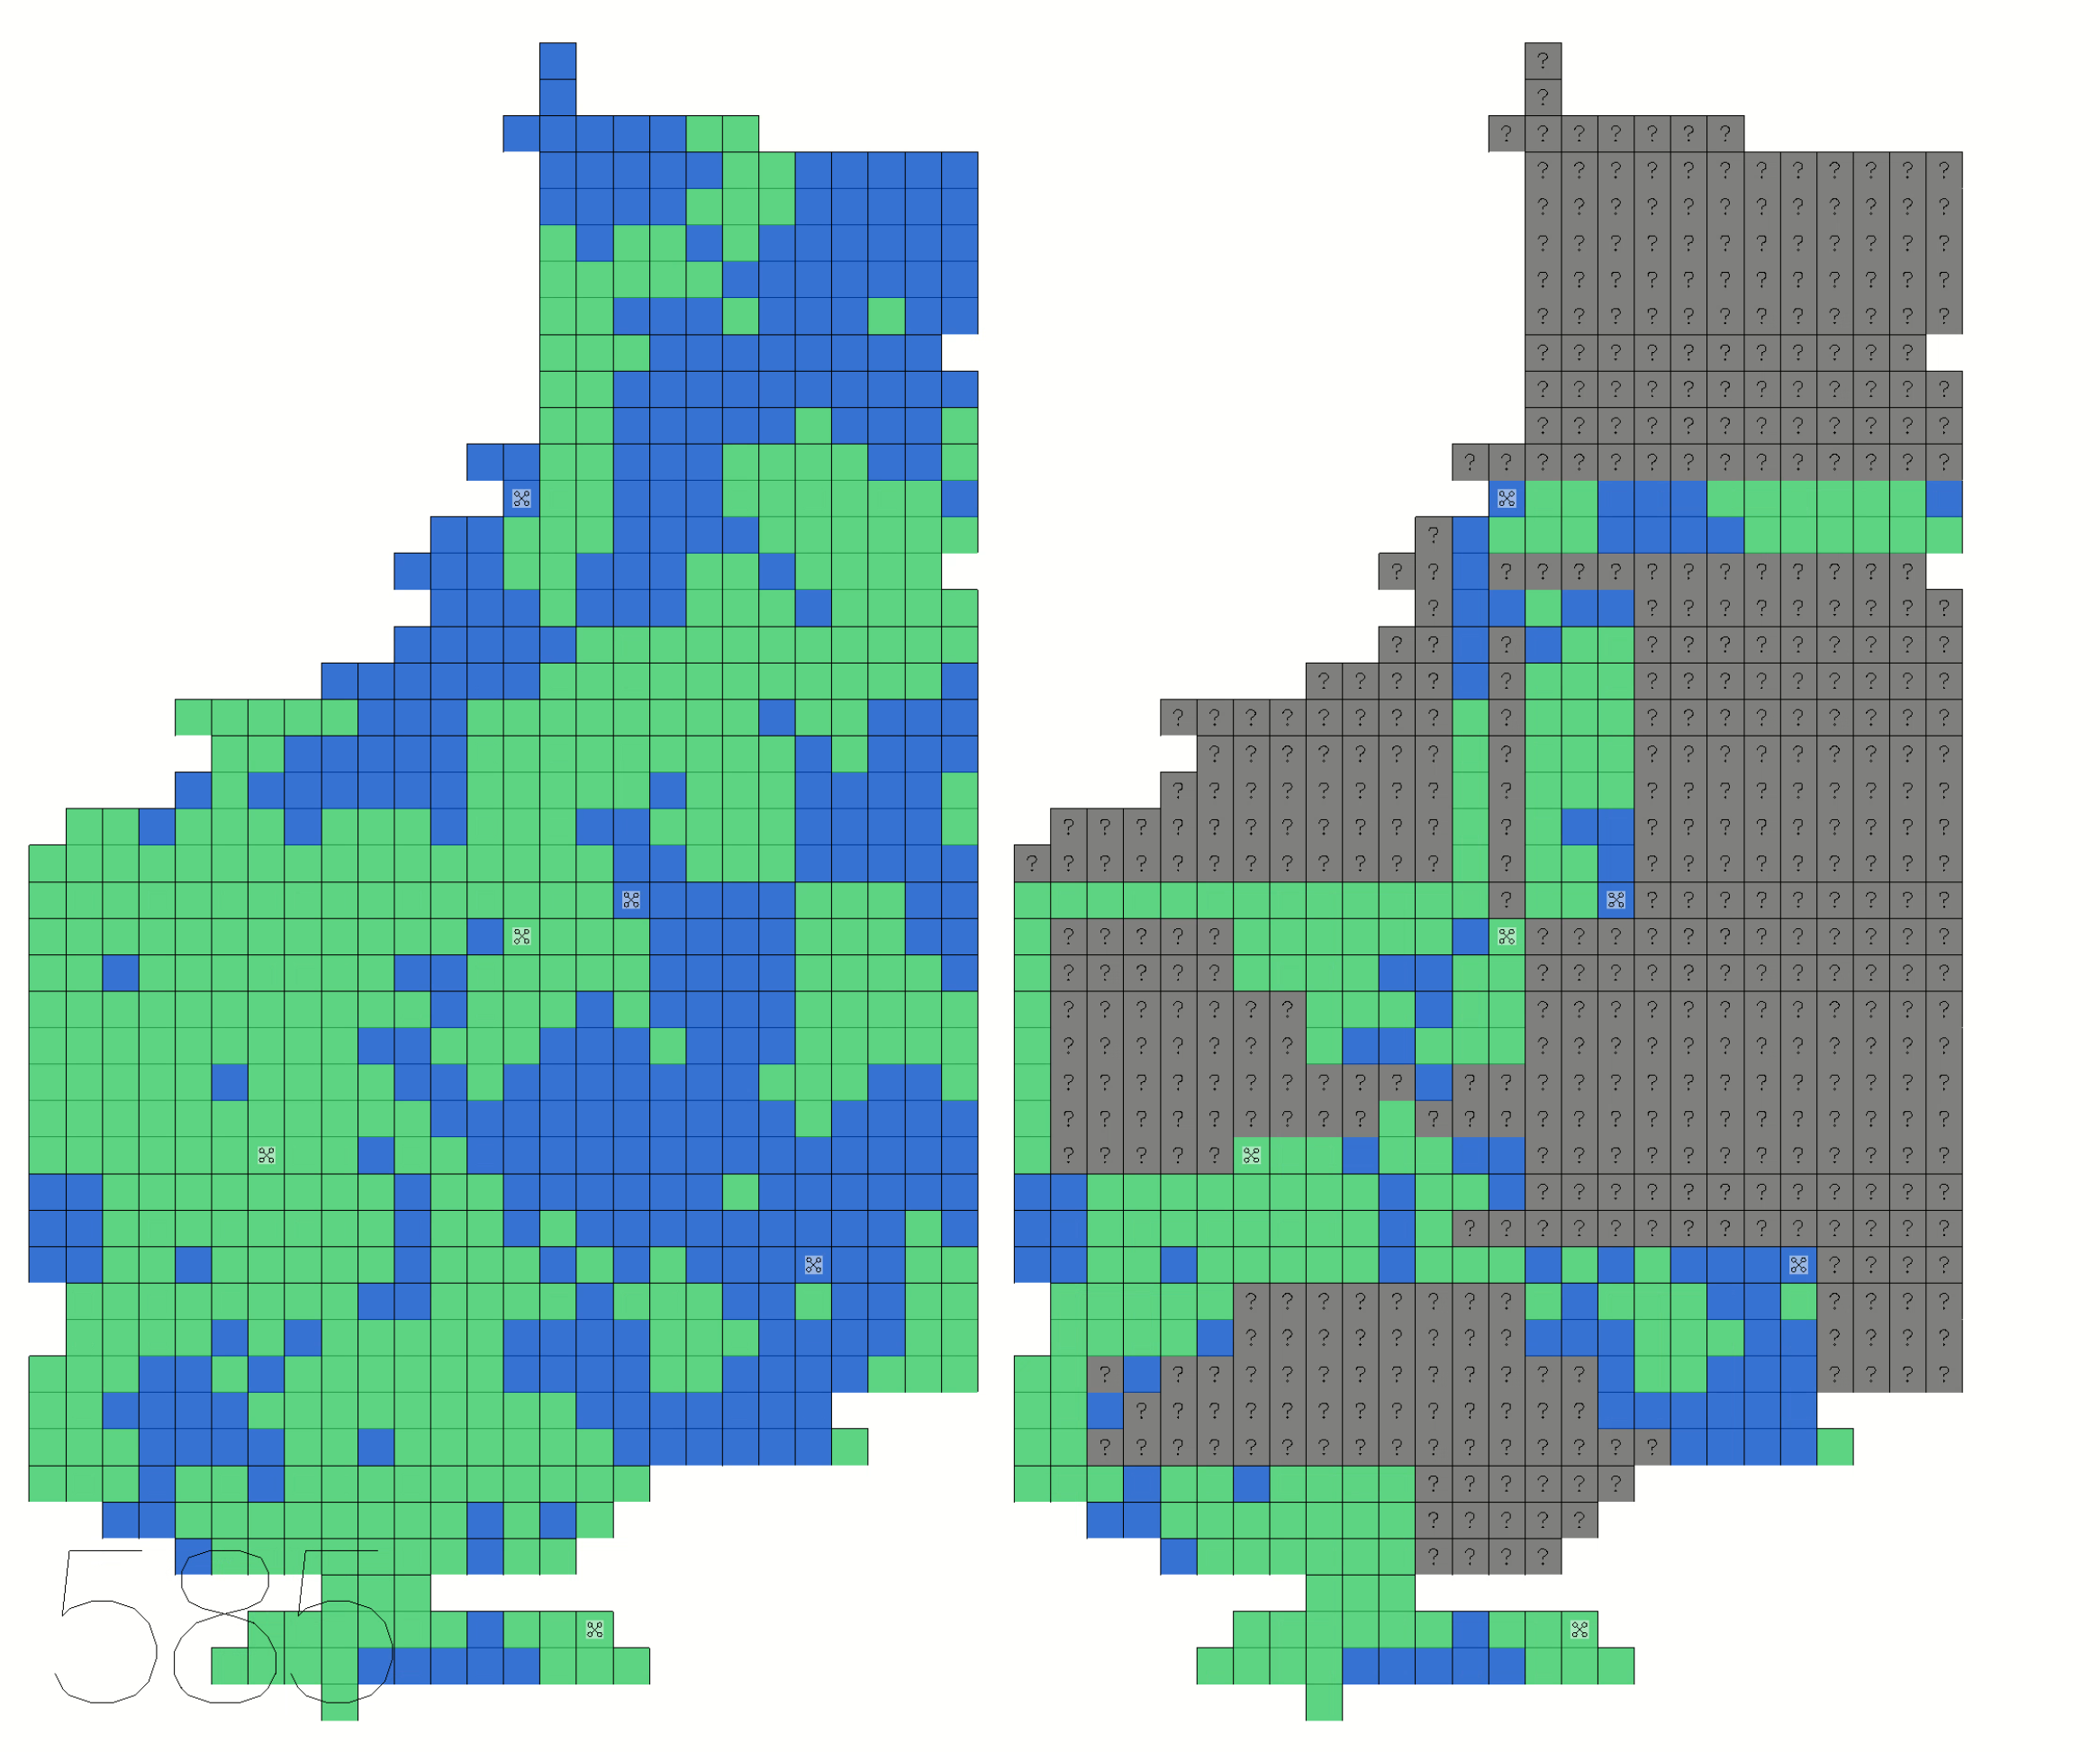
\includegraphics[width=\textwidth]{samplePic}
\caption[Sample Environment Visualization]{A sample environment (left) and the partial information available to robots exploring this environment (right).}
\label {fig:SampleViz}
\end{figure}

\section{Implementation of Problem Statement}

\subsection{Simulated Environment \& Dynamics}

The oprc\_env package represents a multi agent coverage problem as a simulation in which all times and locations are represented with integer values. All ground positions in the environment are indexed by a pair of integers $ (x, y) $. For ease of communication, the $x$ and $y$ coordinates are assumed to correspond to longitude and latitude, respectively. For example, the position $(2, 1)$ is directly east of the position $(1, 1)$, and the position $(0, 0)$ is to the southwest of $(1, 1)$. The minimum x and y coordinates in an environment are both 0 by default, although this is not guaranteed to be true in general. All simulations start at time T = 0.

This design choice allows for simulations to be computed and performance to be evaluated more efficiently than if the environment was modeled as a continuous area or if the dynamics were modeled with continuous time. Since this work claims to achieve coverage paths that are applicable to continuous environments, as was the case with STC and other closely related algorithms, the use of a discrete simulation requires some justification. The work by Gabriely and Rimon on STC provides the inspiration and precedent justification for this choice \cite{STC}. Because all robots following STC move directly between the centers of adjacent cells, it is possible to encode the continuous path followed by an STC-controlled robot as a sequence of environment cells (or subcells, in keeping with the original work's terminology) visited. Since these cells are aligned with a square grid, it is trivial to show that these cells can be indexed by pairs of integer coordinates.

From there, assuming that time is divided such that all drone motions take an integer number of time steps allows for discrete time in simulation. While the ratio of distances corresponding to a cardinal and an intercardinal motion is technically irrational, it is perfectly reasonable to approximate this ratio as 10:14. As long as two drones in the same scenario don't use wildly different proportions of cardinal and intercardinal movements over any extended period, paths that take an equal amount of time in simulation will take a roughly equal amount of time in a continuous environment. Furthermore, the best performing algorithms to solve these scenarios use online techniques that would readily adapt to the occasional one time step delay of move completion. More details on these algorithms can be found in the remaining chapters.

The physical environment of each coverage scenario represents the locations that are in bounds, the level of detailed scrutiny required to cover each of those locations, and the positions of obstacles inside the environment. This is achieved by a map from Position to Patch, where a Patch can represent an environment cell that requires observation at a particular level of detail. This level of detail can be either Close or Far. Patches that require Close detail must be observed by a drone flying at a Low altitude in order to be considered covered, while patches that require only Far detail will be covered once observed by a drone flying at either a High or Low altitude.

%code snippet with Environment definition could go here

Each Patch in an environment can have up to eight neighbors. Four of these neighbors are adjacent to the patch in the four cardinal directions {North, East, South, West}, while the remaining four share a vertex with the patch and lie in one of the four intercardinal directions {NE, SE, NW, SW}. Given an in-bounds location, any arbitrary subset of these eight neighboring locations may be in bounds.

%cover drone, ensemble, all the way through ensemblestatus

\subsection{Environment Interface}

At any given time during an in-progress coverage scenario, only a limited subset of environment information is made available to the algorithm that controls drone motions. The set of in bounds locations in the environment, also known as that environment's \textit{Footprint}, is always known. The partial information available to an agent is represented by the EnvironmentInfo datatype, and this type contains a map from Position to PatchInfo. The set of Position values in this map's domain is normally the same Footprint that belongs to the real environment. A PatchInfo represents a state of knowledge about the patch at a particular location. Patches can be Unseen, Classified, or FullyObserved. As the names suggest, Unseen and FullyObserved correspond to patches that have never been seen at all and to patches that have been completely covered, respectively. A Classified patch is one where the level of observation detail required (DetailReq) is known, but the patch has not been fully covered yet. In practice, this only comes up for patches that require Close scrutiny and have only been seen by one or more drones flying at a High altitude, in which case the patch would have only been observed with Far scrutiny.

The EnvironmentInfo datatype, together with the previously described EnsembleStatus, forms the content of the WorldView datatype. A WorldView represents all of the information about the current state of the simulation available to a control algorithm. Control algorithms plug in to the simulation via an instance of the Policy typeclass, which abstracts the behavior of any type capable of commanding directions to an Ensemble and potentially maintaining a notion of internal state. Specifically, the typeclass is defined as:

\begin{minted}{haskell}
class Policy p where
  nextMove :: p -> WorldView -> (NextActions, p)
\end{minted}

As the name suggests, NextActions is a datatype that expresses newly issued commands for some drones to follow. This is implemented as an association list:

\begin{minted}{haskell}
type NextActions = [(Drone, Action)]
\end{minted}

The nextMove function provided by any type $p$ with an instance of Policy is called by the core simulation code to determine what moves have been commanded to each drone in the simulation at every time step. As suggested by the type signature, most sensible implementations of nextMove use a particular value of the policy type $p$ to decide what moves to command next. A simple type for which a Policy instance would be easy to provide might contain a direct mapping from WorldViews to NextActions. In this case, an instance of nextMove would determine what value of NextActions to return by simply performing a lookup on this map at each time step. Along with this value, nextMove would return the original policy value along with the result of that map query. 

Of course, an instance of Policy like the one described above is not easy to implement for anything but the smallest environments and number of drones. This is because the number of possible WorldViews in an environment must be larger than the number of ways the drones can be distributed in that environment. It is easy to show that the latter notion corresponds to sampling from a bag of unique outcomes with replacement. Thus, for an environment with $n$ cells and $m$ drones, the number of WorldViews is much greater than $n^m$. This is already an inconvenient number of entries to store in a data structure, and each of these outcomes corresponds to a distribution of drones in space that is achievable. As a result, some number of entries for each of these would need to be included in any Policy implemented as a lookup table.

Counting the number of achievable WorldViews exactly, complete with all of the possible partial information states, is much more difficult. However, the established lower bound makes it clear that this quantity is not practical to handle in any direct way. This discussion may seem pointless for an implementation of Policy that is obviously unwise. However, getting a sense of this scale has implications that will inform the design of internal representations used by more effective Policy instances as discussed in later chapters. Luckily, because nextMove yields another value of p along with its NextActions decision, it is possible and often desirable for p to encode a control strategy that learns and plans, evolving with the context in which it currently operates.

Some control algorithms are capable of learning from experience and modifying behavior in a given simulation based on results from a previous one. The PersistentPolicy typeclass exists in order to provide the interface required for this functionality:

\begin{minted}{haskell}
class Policy p => PersistentPolicy p where
  cleanup :: p -> (WorldView -> p)
\end{minted}

The exact purpose of cleanup's type may not be immediately apparent. In short, the most useful policy representations tend to need access to some information about the current environment before they can be initialized. The function type of cleanup's output shows that it will return the right kind of value to make this initialization fit nicely with tooling developed for more general Policy instances. The fact that cleanup must be applied to a value of type p before it returns this value allows control algorithms to pass any encoded strategies learned during task execution to be applied to the completion of the next task. As later chapters will discuss, this capability is actually necessary for optimal performance when the distribution of environments is not known before task execution begins.

\subsection{Environment Generation}

In order to evaluate the coverage performance of any agent with a Policy instance, it is necessary to have a simulated environment for that algorithm to cover. It is also useful to have a large dataset of simulated environments for the agent to cover when collecting performance statistics. Finally, since some Policy instances may be capable of learning and specializing their behavior to the distribution of environments previously explored, it is useful to have fine control over the nature of the environments in a particular dataset. To meet all of these needs, \textit{oprc\_env} has a utility executable called \textit{generate\_environments} to create custom environments and environment datasets based on a specification of the distribution from which those environments should be drawn.

Before describing the capabilities of \textit{generate\_environments} in full, it is useful to consider the algorithms used to generate one specific environment. There are a few different algorithms for this purpose, and each one generates environments from a distribution that is qualitatively different from the others.

The simplest environment generation algorithm to describe is called the \textit{BernoulliGen.} As the name suggests, this generator samples a required level of scrutiny from the same Bernoulli distribution for each location in the generated environment's Footprint. As a result, most of the content of the \textit{BernoulliGen} algorithm comes from the procedure used to generate Footprints. The \textit{randomFootprint} function supplies this functionality.

The \textit{randomFootprint} algorithm generates a Footprint, or set of in-bounds locations. While a Footprint alone does not constitute a usable coverage environment, it can be augmented to form a complete environment description by algorithms that assign a DetailReq value to each of the positions in the set. The type signature and corresponding parameter nicknames used by randomFooprint are as follows:

\begin{minted}{haskell}
randomFootprint :: StdGen --a source of randomness
                -> Int --allowed variation between border locations
                -> Int -> Int -> Int -> Int --coordinate limits for Positions
                -> Maybe Footprint
randomFootprint gen 
                varLimit 
                xMin xMax yMin yMax =
  undefined --bulk of implementation excluded for brevity
\end{minted}

Roughly, this function randomly selects one point on each face of the ``bounding box" of legal position coordinates defined by the x/y min and max arguments. Then, interpolation is used to connect turn these points into a discrete approximation of a quadrilateral. Each coordinate on this perimeter is randomly perturbed by an amount whose magnitude must not exceed varLimit. Finally, the set of all positions inside this perimeter is computed and returned. The output type of a fully applied randomFootprint, Maybe Footprint, indicates that this function may fail to produce a valid Footprint. This is because the arguments for randomFootprint are sometimes sourced from configuration files or user input, and information from these sources may correspond to unrealizable requirements.

In addition to this basic footprint generation function, it is possible to augment the complexity of the generated footprints by taking some locations out of bounds. One simple algorithm for this purpose creates the set of all locations whose Chebyshev distance from some center location is no greater than some limiting value. However, careless use of such a function can lead to unintended consequences. For example, if the group of locations taken out of bounds includes one or more positions that were already on the perimeter of a Footprint, the resulting Footprint will not have a distinch cluster of out of bounds locations in the middle of an in bounds region. Since taking locations out of bounds is primarily useful for simulating obstacles in an environment, this is usually not a desirable result. Even worse is the case where the group of locations taken out of bounds intersects with multiple non-adjacent sections of the original Footprint's perimeter. In this case, the connectivity of the resulting environment could be changed such that a drone starting in one set of patches has no way of visiting the other set. This makes performance of complete coverage impossible, so this is almost always undesirable.

The main function used to take locations out of bounds, \textit{hole}, implements a simple safeguard to avoid these pitfalls: it takes away positions in groups organized by ascending Chebyshev distance from the center. Starting from the cetner itself ($d = 0$), this procedure repeatedly removes another ring-shaped layer of locations until one of two things happens. The function can either reach the desired threshold for distance from the center, or it can detect that removing another layer would cause the removal of a border position. In either case, the algorithm terminates. With these safeguards in place, \textit{hole} can be used to scatter virtual obstacles around an environment at different positions and with different obstacle sizes. 

Given a random Footprint, the remainder of BernoilliGen simply assigns a DetailReq value to each location in the Footprint independently. The specific value assigned to each patch is determined by sampling a floating point number from the interval [0, 1] and then comparing this value to a threshold provided as input to the function. The value of this threshold corresponds to the probability that any individual patch will be assigned the value Close, meaning that it must be observed by a Low drone before it is covered.

Other algorithms available for use with \textit{generate\_environments} produce an Environment in which the spatial distribution of DetailReq values features regions that are locally correlated in some way. A variety of these algorithms exist, and all of them rely on \textit{randomFootprint} for the environment's basic shape. From there, however, these algorithms rely on procedures for filling in DetailReq values which are more sophisticated than the one used by \textit{BernoulliGen}. In order to produce a somewhat structured ouput that still features randomness, many of these algorithms benefit from an efficient way of assigning DetailReq values to patches in a random order. This allows each new assignment to be drawn based on the presence of any other locations that have already been filled in.

The Fisher-Yates shuffle is an algorithm to reorder, or shuffle, the elements of a finite sequence. This algorithm provides a random reordering of a list of positions to support the many environment generation algorithms that require this functionality. It is also used for implementation of random drone failure and other simulation features that have not yet been described. It is possible to run this algorithm in-place on a sequence of length n in $O(n)$ time. In addition, given a way to randomly select an element from a range of integers with uniform probability, the Fisher-Yates shuffle has the useful property of producing any possible reordering of the sequence with uniform probability. The original work by Richard Durstenfeld to develop this algorithm for use on a computer can be found in \cite{FYShuffle}. The version presented here is a generalization of that algorithm to operate directly on sequences of arbitrary data.

The \textit{Shuffle} function assumes access to a function $g$ that can accept an integer argument $i$ and return an integer sampled uniformly from 0 to i, inclusive. It operates on $l$, a finite sequence of values of any datatype. For simplicity, it also assumes access to functions that get the length of a finite sequence and swap the elements of that sequence at two indices. Finally, note that sequence indexing starts at 0.

\begin{algorithmic}

\Function{Shuffle}{$g, l$}
  \State $n\gets length(l)$	
  \While{$n > 0$}
      \State $s\gets g(0, n)$
      \State $swap(l, s, n)$
      \State $n\gets n - 1$
  \EndWhile
  \State \Return $l$
\EndFunction

\end{algorithmic}

The actual source code for this algorithm can be found in the FisherYatesShuffle module in \textit{oprc\_env}.

Using the Fisher Yates shuffle, it is possible to create environment generation algorithms that tend to output locally correlated "clusters" of similar patches. Each patch in the environment is given a DetailReq value by taking a supplied threshold value and altering that value by a small amount for any neighboring patches that hae already been given an assignment. Each of these threshold alterations makes it slightly more likely to generate a patch of the same type as the one that triggered the alteration. The order in which patches are filled in is determined by applying the Fisher Yates shuffle to a list of all in bounds locations in the environment. This order randomization step makes it likely that a small number of completely unbiased "seed" locations will get a DetailReq value sampled that is not affected by any neighbors. Depending on the exact parameters used, skipping this randomization step may result in environments that are dominated by one scrutiny requirement even when the initially supplied threshold value is not biased one way or the other.

\section{Operation and Software Utilities}

\subsection{Running Simulations}

The Scenario type and the functions that operate on it are responsible for expressing and updating the state of a simulation. The type itself consists of a WorldState and a Policy for tracking the instantaneous state of the simulation, along with time and history parameters to allow simulation replays and performance analysis:

\begin{minted}{haskell}
data Scenario p =
  Scenario {
    getPolicy :: p
  , getWorldState :: WorldState
  , getTime :: Integer
  , getHist :: MoveHistory
  }
\end{minted}

The function that steps simulations forward in time takes any \verb|(Policy p => Scenario p)| and applies nextMove to that Scenario's Policy and a WorldView generated from the current WorldState. The resulting policy is assigned to the next Scenario value. The NextActions portion of nextMove's output is where most of the simulation's portion of the computation occurs. First, for replay and analysis, any newly commanded actions are added to the MoveHistory. In addition, time is incremented.

A function, \textit{updateState}, figures out the new instantaneous WorldState from

\subsection{Visualization Tools and Parsing}

The most precise human-friendly way to communicate the activity of this simulation is via text written to the terminal by the various executable functions in \textit{oprc\_env}. Within this project, the typeclasses \textit{Show} and \textit{Pretty} must be provided for values of a particuar datatype to be expressed in this way. Between these two typeclasses, \textit{Show}'s instances tend to provide completely unambiguous and easily parseable representations of data. This is very convenient for some datatypes, such as \textit{Hop}, where the bare programming language syntax is adequate for expressing such a simple idea in a form humans can understand at a glance. For example, a hop 3 positions east and one position south would be printed to the console as (3, -1) when using \textit{Show}.

\textit{Pretty} is at its most useful when expressing data of an intermediate level of complexity. Data that is list-like, that has two or three levels of hierarchy, or that is otherwise large but mostly one-dimensional is not well suited to expression in the raw programming syntax that could, in principle, be used to specify such values directly in source code. While it may be possible to write Show instances that do an adequate job of expressing this kind of code, it is not straightforward to derive easily readable \textit{Show} instances for large datatypes in terms of the instances of suboordinate datatypes, which may have layers of hierarchy even before being included in the parent datatype. For example, indenting the contents of some string representing an already hierarchical datatype to fit inside a larger string with yet another layer would require meaningful parser development for every new instance of \textit{Show}. Furthermore, while Show instances may compute arbitrarily sophisticated String values for the data they represent, convention dictates that instances should be expressed with the syntax required to directly program those values elsewhere. \textit{Pretty} solves these problems by representing the hierarchical nature of its contents explicitly, rather than with repeated newline and tab characters or with nested delimiters in a string. In addition, the functions used to get these representations on a screen make rich use of IO such that they can adapt a presentation of data to fit on terminal windows of various sizes. This allows the contents of very small values of complex datatypes such as Scenario to be displayed on screen in a way that is easy to program and to understand.

However, the coverage behavior computed in these simulations can be difficult to interpret when expressed \textit{exclusively} in terms of words and numbers. Because this software simulates the exploration of two dimensional worlds, some of the datatypes are best expressed in a medium better suited to expressing two continuous dimensions of data. While this kind of expression is less precise and less suitable for low-level debugging tasks than text representations, it enables an immediate and intuitive understanding of large quantities of data being updated on screen at up to 60 frames per second. To facilitate the design and presentation of such data, this software makes use of the \textit{Gloss} graphics library.

The animation software developed for \textit{oprc\_env} is primarily for visualizing environments with color coded two-dimensional drawings. An environment is displayed as a collection of colored squares. Each square in this collection represents the patch type associated with one position. All of these squares appear in grid aligned positions that are filled in with white wherever there is no in-bounds patch. In addition to empty environments, EnvironmentInfo data can be displayed. This datatype represents the state of partial information about an environment. Fully known EnvironmentInfo patches are drawn the same as they would be in an environment. Locations that are unobserved are drawn in grey with the question mark (?) character overlaid to indicate uncertainty. Partially observed patches are always classfied by required scrutiny, so these are partitioned into a grey triangle and a triangle of whatever color corresponds to the fully observed patch.

Often, it is useful to visualize both the plain enivironment and the partial information known by a policy about that environment at the same time. The most common visualization used in this software shows an environment on the left and the information used by a policy on the right. In addition, the status of any drones in the environment are represented with symbols overlaid on the appropriate locations within the EnvironmentInfo representation. Finally, a timer appears in the lower left corner (Figure \ref{fig:VizDemo}).

\begin{figure}[H]
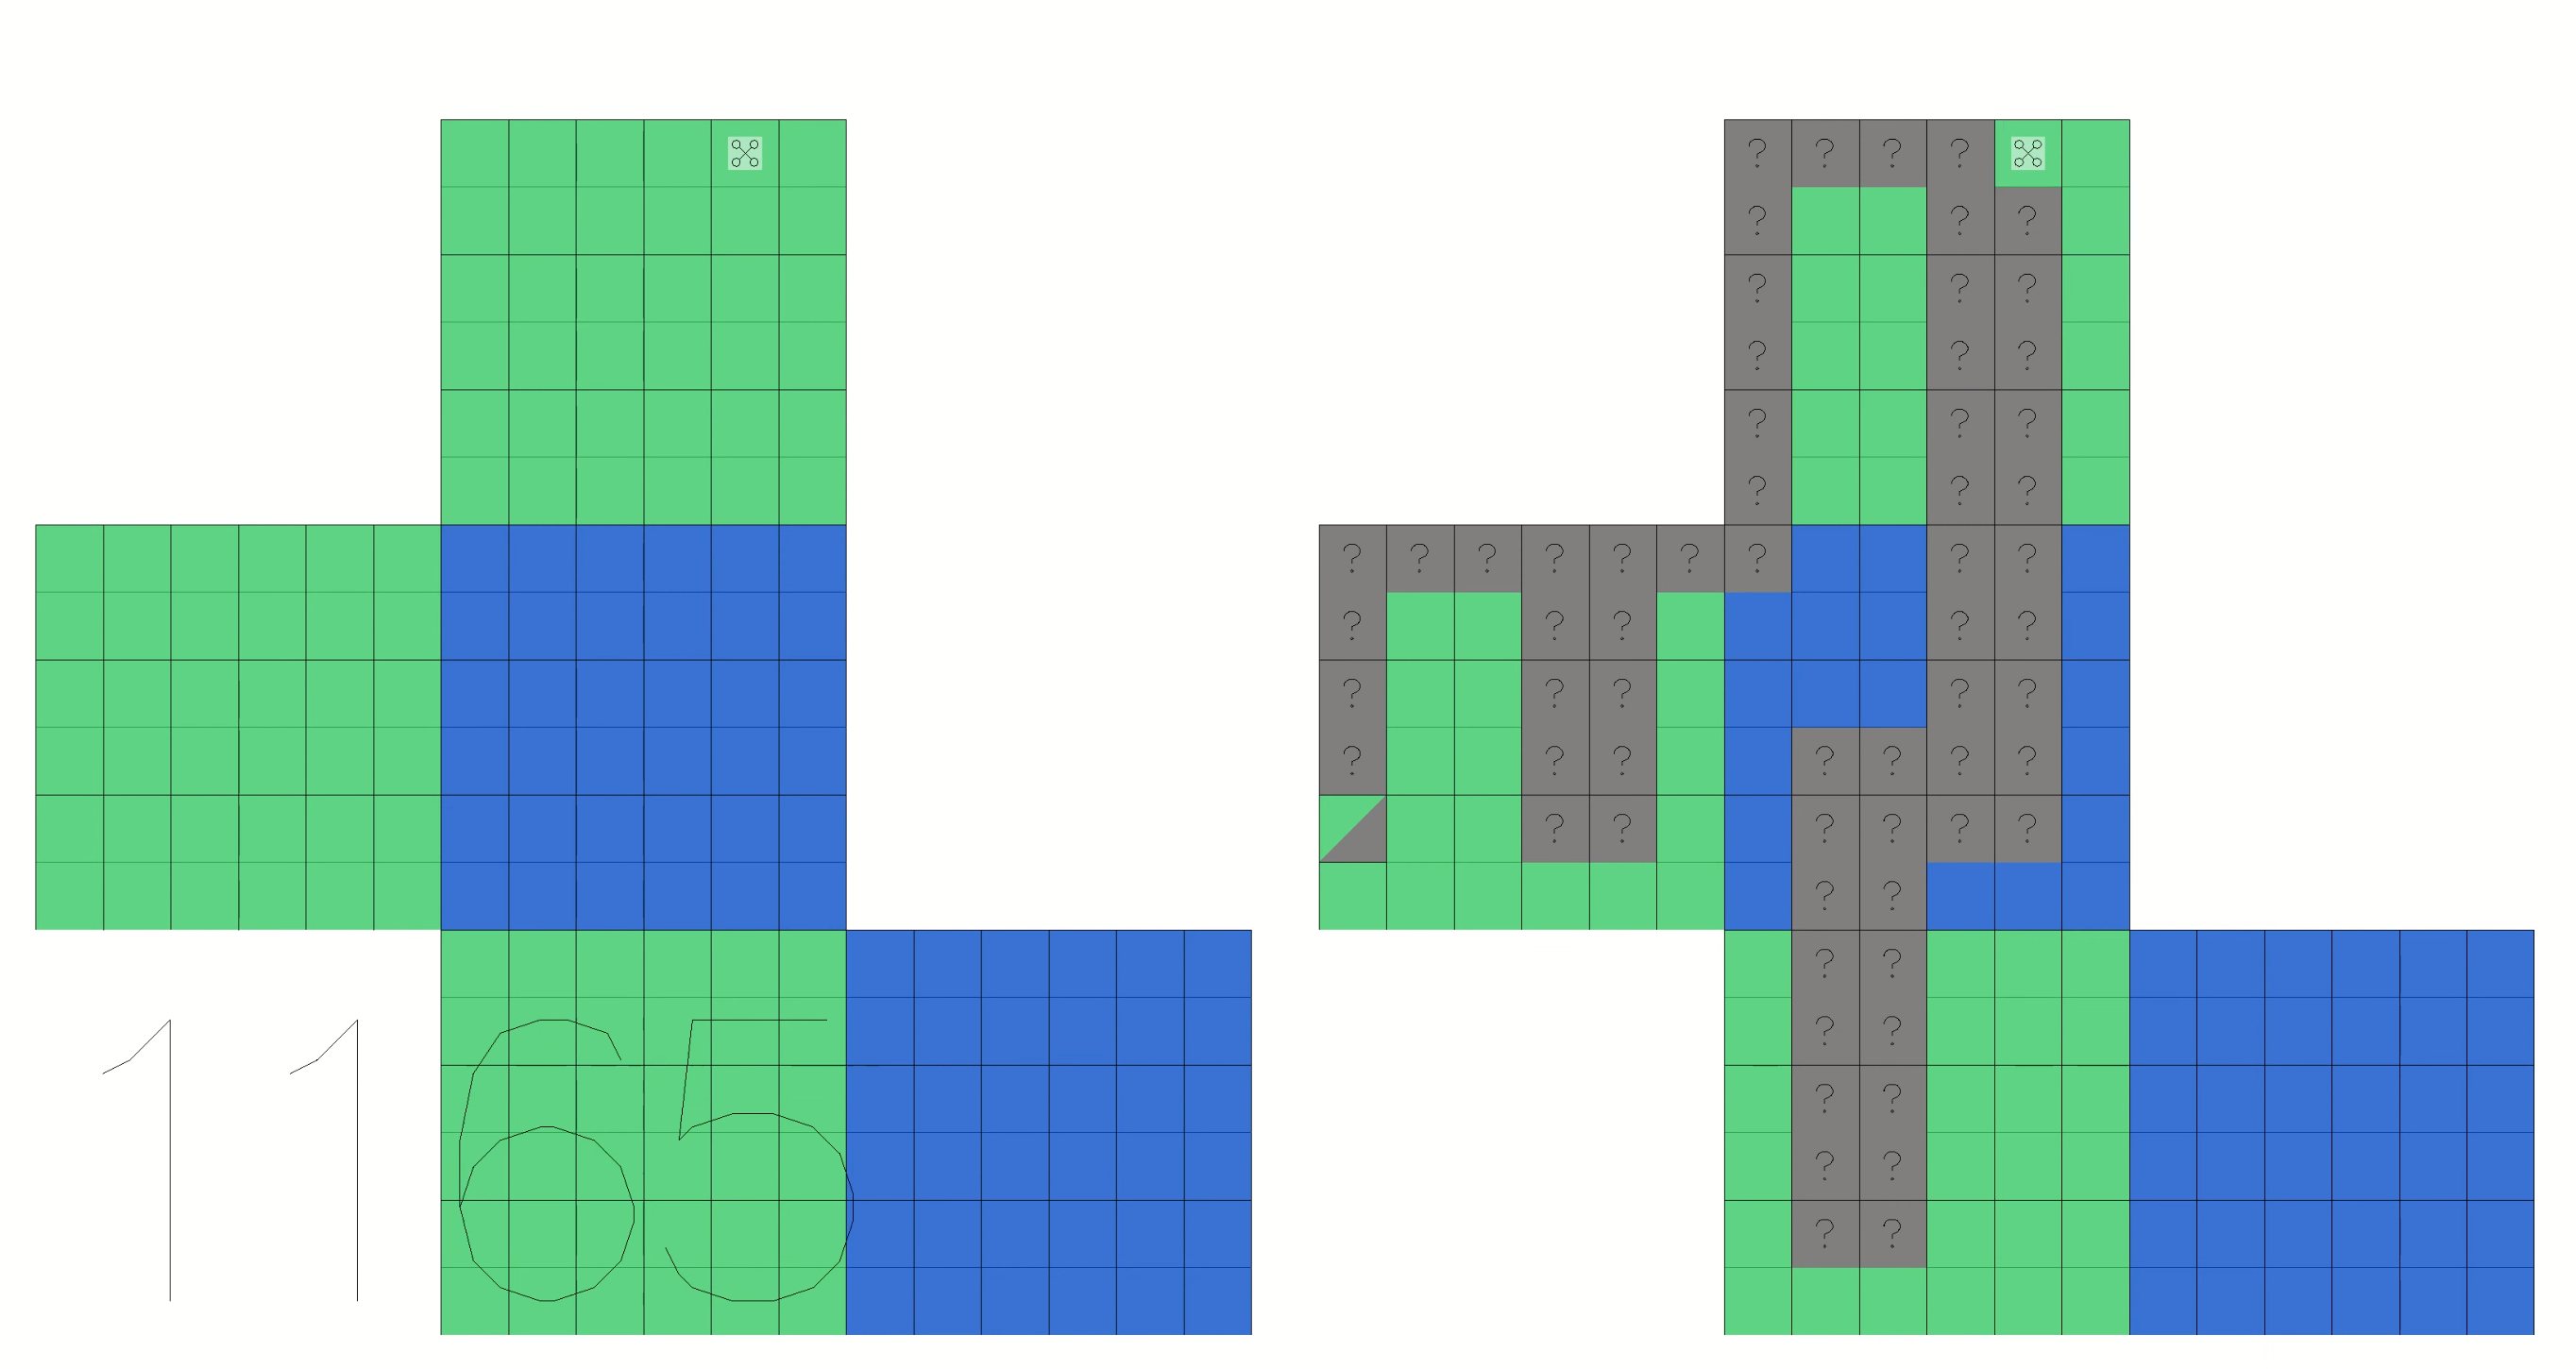
\includegraphics[width=\textwidth]{visualizationDemo}
\caption[Visualization of a Small Environment During Coverage]{A sample environment (left) appears next to a visualization of the active coverage task (right). Univisited locations are marked in grey on the right. A pictograph made of crossed lines with circles on the ends depicts the drone and shows its loation on the map. The only partially observed location on the map appears on the west end of the EnvironmentInfo representation, and is partially covered by a grey triangle.}
\label {fig:VizDemo}
\end{figure}

The modules containing this animation code, \textit{AnimateReplay} and \textit{AnimateScenario}, also provide functionality for drawing some of the data structures used by particular Policy instances. Some of these data structures can be thought of as walls for the drones to follow in a loop, and so are suitable for drawing over a map. For more information on this, refer to the next two chapters.

\textit{oprc\_env} also features significant parsing functionality. This functionality is useful for creating custom environments to load and run in the simulation, serializing and saving a collection of automatically generated environments for evaluating the performance of some policy, and allowing an executable to understand interactive input of control commands. The parsing used in this code does not occur in any speed critical areas, and so the best library for the job should emphasize ease of use over speed. Because of that, the Trifecta library by Edward Kmett is used here. This library provides monadic parser combinators and makes it very easy to sort through descriptions of datatypes in plain text input to a console, etc. The slightly more complex parsing involves reading in environment configuration files. However, the resulting parser makes it possible to work with a representation of environments that is very easy for humans to read and write. For example, the following file comes from a plain text configuration that corresponds to the environment used in Figure \ref{fig:VizDemo}:

\begin{verbatim}
      HHHHHHLLLLLL
      HHHHHHLLLLLL
      HHHHHHLLLLLL
      HHHHHHLLLLLL
      HHHHHHLLLLLL
      HHHHHHLLLLLL
HHHHHHLLLLLL      
HHHHHHLLLLLL      
HHHHHHLLLLLL      
HHHHHHLLLLLL      
HHHHHHLLLLLL      
HHHHHHLLLLLL      
      HHHHHH      
      HHHHHH      
      HHHHHH      
      HHHHHH      
      HHHHHH      
      HHHHHH      
\end{verbatim}

Note that the plain text representation of an environment appears vertically flipped when compared with the resulting environment visualization. This is an intentional trade off that makes the line numbers of a plain text file correspond to the y coordinate of any patches specified on that line. Because many modern plain text editors track both the line number and character position of a cursor, this makes it possible to easily specify environments with properties that change at precise coordinates. Other than that exception, it should be easy to see the correspondence between this plain text and the final illustrated environment on the left of \ref{fig:VizDemo}.

\section{Extra Features}

\subsection{Drone Dropout}

In order to fully test the adaptability of Policy implementations, \textit{oprc\_env} includes functionality to run simulations with drone droupout. When this feature is in use, up to one drone may be permanently disabled at each time step in the simulation. Whether or not a drone drops out during a given time step is based on comparison of a random number sampled from the uniform distribution over the interval [0, 1] and a customizable threhold value. It is not possible for more than one drone to fail during a single moment in time according to this formulation. Also, in order to make sure that all scenarios are possible to complete, at least one drone is guaranteed to be operational at all times. These two assimptions and the basic model of drone dropout they apply to are not meant to be especially realistic. However, this model of dropout is sufficient for splitting Policy algorithms into a few coarse categories according to adaptability: those that fail when dropout occurs, those that complete a dropout scenario in an inefficient way, and those that smoothly adapt to each dropout event they occur. Note that animations of scenarios with dropout do not show disabled drones in a unique way. Rather, disabled drones are simply frozen in place with whatever state they had just before beind disabled. Theoretically, this makes it difficult to distinguish between a disabled drone and one which is active but repeatedly receiving Hover commands. However, this issue does has not come up in practice.

%include a video of the simulation using the media9 tool? This may not have widespread support in pdf viewers though
%https://www.ctan.org/tex-archive/macros/latex/contrib/media9